\include{preamble-libroEstGrado0-minimizarPags.tex}
\title{Matemáticas Ilustrativas\\
{\large Grado 0 - Unidad 1}}
\author{Adaptación del Grupo LEMA\\
\href{https://www.grupolema.org}{\nolinkurl{https://www.grupolema.org}}
}
\date{March 18, 2025}
\begin{document}
%% bottom alignment is explicit, since it normally depends on oneside, twoside
\raggedbottom
%% Target for xref to top-level element is document start
\label{gra0-uni1}\hypertarget{gra0-uni1}{}
\maketitle
\thispagestyle{empty}
\renewcommand*{\abstractname}{}
\begin{abstract}
Este documento (HTML, pdf, latex o epub) se generó con \href{https://pretextbook.org}{PreTeXt}\footnote{\nolinkurl{pretextbook.org}\label{meta-source-2-2}}. El código fuente con el contenido para generarlo se encuentra en \href{https://github.com/enriqueacosta/IllustrativeMath-GrupoLEMA}{\nolinkurl{github.com/enriqueacosta}}.%
\end{abstract}
\clearpage
\renewcommand*{\abstractname}{Licencia}
\begin{abstract}
\justifying
2024~Versión PreTeXt, traducciones completas de las guías y adaptaciones © Enrique Acosta (\href{https://enriqueacosta.github.io}{\nolinkurl{enriqueacosta.github.io}}). Iniciativa del Grupo LEMA (\href{https://www.grupolema.org}{\nolinkurl{www.grupolema.org}}). Publicado bajo una licencia Creative Commons {\em Attribution NonCommercial ShareAlike} 4.0 International (CC BY SA NC 4.0).%
\par
En breve e incompleto (los detalles están en las licencias), \alert{tiene toda libertad para adaptar, copiar y distribuir este material siempre y cuando le mantenga la misma licencia, incluya la atribución correspondiente (mencione a Enrique Acosta, al Grupo LEMA, a Illustrative Mathematics y a OpenUp Resources en la forma que se describe a continuación) y lo use para fines no comerciales}.%
\par
Ver detalles de la licencia en \href{https://creativecommons.org/licenses/by-nc-sa/4.0/}{creativecommons.org}\footnote{\nolinkurl{creativecommons.org/licenses/by-nc-sa/4.0/}\label{meta-copyright-6-2}}.%
\par
Además, se permite la impresión y distribución a costo para uso educativo o personal. La reventa comercial o actividades con fines de lucro no están permitidas sin autorización previa.%
\par
Grados K-5 adaptados de IM K–5 Math v.I, ©~2021 Illustrative Mathematics~® \href{https://curriculum.illustrativemathematics.org}{illustrativemathematics.org}\footnote{\nolinkurl{curriculum.illustrativemathematics.org}\label{meta-copyright-8-4}} en su versión en español en \href{https://im.kendallhunt.com/K5_ES/curriculum.html}{im.kendallhunt.com}\footnote{\nolinkurl{im.kendallhunt.com/K5_ES/curriculum.html}\label{meta-copyright-8-6}}, distribuido con una licencia Creative Commons Attribution 4.0 International License (CC BY 4.0). Ver detalles de esta licencia en \href{https://creativecommons.org/licenses/by/4.0/}{creativecommons.org}\footnote{\nolinkurl{creativecommons.org/licenses/by/4.0/}\label{meta-copyright-8-8}}.%
\par
Grados 6-8 adaptados de IM 6–8 v3.1415, ©~2019 Illustrative Mathematics~® \href{https://curriculum.illustrativemathematics.org}{illustrativemathematics.org}\footnote{\nolinkurl{curriculum.illustrativemathematics.org}\label{meta-copyright-9-4}} en su versión en español en \href{https://im.kendallhunt.com/K5_ES/curriculum.html}{im.kendallhunt.com}\footnote{\nolinkurl{im.kendallhunt.com/K5_ES/curriculum.html}\label{meta-copyright-9-6}}, distribuido con una licencia Creative Commons Attribution 4.0 International License (CC BY 4.0), a su vez ©~2017-2019 Open Up Resources 6–8 Math v2, disponibles en \href{https://openupresources.org/math-curriculum/}{openupresources.org}\footnote{\nolinkurl{openupresources.org/math-curriculum/}\label{meta-copyright-9-9}}, con la misma licencia (CC BY 4.0). Ver detalles de esta licencia en \href{https://creativecommons.org/licenses/by/4.0/}{creativecommons.org}\footnote{\nolinkurl{creativecommons.org/licenses/by/4.0/}\label{meta-copyright-9-11}}.%
\par
\alert{Nota:} Las traducciones anteriormente mencionadas fueron lideradas y coordinadas por miembros del Grupo LEMA. Ver detalles en:%
\begin{itemize}[label=\textbullet]
\item{}K-5: \href{https://curriculum.illustrativemathematics.org/k5/teachers/grade-1/course-guide/contributors.html}{illustrativemathematics.org}\footnote{\nolinkurl{curriculum.illustrativemathematics.org/k5/teachers/grade-1/course-guide/contributors.html}\label{meta-copyright-10-2-1-2}}%
\item{}6-8: \href{https://curriculum.illustrativemathematics.org/MS/teachers/1/contributors.html}{illustrativemathematics.org}\footnote{\nolinkurl{curriculum.illustrativemathematics.org/MS/teachers/1/contributors.html}\label{meta-copyright-10-2-2-2}}%
\item{}\href{https://enriqueacosta.github.io/blog/es/posts/translating-im/}{enriqueacosta.github.io}\footnote{\nolinkurl{enriqueacosta.github.io/blog/es/posts/translating-im/}\label{meta-copyright-10-2-3-2}}%
\end{itemize}
%
\parbox{\linewidth}{%
Este material incluye imágenes con licencias abiertas que tiene copyright de sus respectivos autores. Estas imágenes mantienen los términos de sus propias licencias de uso. Ver detalles en la sección de atribuciones de imágenes.%
}
\end{abstract}
\clearpage
\renewcommand*{\abstractname}{Gracias a ...}
\begin{abstract}
Las siguientes personas aportaron en el desarrollo de esta versión de Matemáticas Ilustrativas.%
\par
Traducción y procesamiento de contenido%
%
\begin{itemize}[label=\textbullet]
\item{}Enrique Acosta Jaramillo%
\item{}Andrés Forero Cuervo%
\item{}Nathaly Otero Paternina%
\item{}Jonathan Defelipe Payane%
\end{itemize}
Revisiones%
%
\begin{itemize}[label=\textbullet]
\item{}Verónica Mariño Salazar%
\end{itemize}
Ingeniería y desarrollo%
%
\begin{itemize}[label=\textbullet]
\item{}Enrique Acosta Jaramillo%
\end{itemize}
Autores (en inglés)%
%
\begin{itemize}[label=\textbullet]
\item{}Illustrative Mathematics. Ver detalles en los siguientes enlaces.%
%
\begin{itemize}[label=$\circ$]
\item{}K-5: \href{https://im.kendallhunt.com/k5_es/teachers/grade-4/course-guide/contributors.html}{https:\slash{}\slash{}im.kendallhunt.com\slash{}k5\slash{}}\footnote{\nolinkurl{im.kendallhunt.com/k5_es/teachers/grade-4/course-guide/contributors.html}\label{meta-contributors-10-1-2-1-2}}%
\item{}6-8: \href{https://im.kendallhunt.com/MS/teachers/2/contributors.html}{https:\slash{}\slash{}im.kendallhunt.com\slash{}MS\slash{}}\footnote{\nolinkurl{im.kendallhunt.com/MS/teachers/2/contributors.html}\label{meta-contributors-10-1-2-2-2}}%
\end{itemize}
\end{itemize}
\end{abstract}
\renewcommand*{\abstractname}{y gracias a ...}
\begin{abstract}
Los distintos formatos de este documento (PDF, LaTeX, EPUB) se generaron utilizando software de licencia abierta desarrollado gracias al esfuerzo de muchas personas. Entre estos destacamos:%
%
\begin{itemize}[label=\textbullet]
\item{}\href{https://pretextbook.org}{Pretext}\footnote{\nolinkurl{pretextbook.org}\label{meta-attributionsOpenSource-3-1-2}}: Sistema para crear y publicar libros de texto, artículos de investigación y monografías, especialmente en disciplinas STEM.%
\item{}\href{https://www.mathjax.org}{MathJax}\footnote{\nolinkurl{www.mathjax.org}\label{meta-attributionsOpenSource-3-2-2}}: Biblioteca JavaScript para mostrar fórmulas matemáticas en cualquier navegador web.%
\item{}\href{https://www.latex-project.org}{LaTeX}\footnote{\nolinkurl{www.latex-project.org}\label{meta-attributionsOpenSource-3-3-2}} y \href{https://tug.org}{TeX}\footnote{\nolinkurl{tug.org}\label{meta-attributionsOpenSource-3-3-4}}: Sistema de preparación de documentos para impresión, ampliamente usado para documentos profesionales.%
\item{}\href{https://ctan.org/pkg/pgf}{TikZ}\footnote{\nolinkurl{ctan.org/pkg/pgf}\label{meta-attributionsOpenSource-3-4-2}}: Paquete de LaTeX para crear gráficos vectoriales de alta calidad, desde diagramas matemáticos hasta ilustraciones técnicas y científicas.%
\item{}\href{https://ctan.org/pkg/fontawesome}{FontAwesome}\footnote{\nolinkurl{ctan.org/pkg/fontawesome}\label{meta-attributionsOpenSource-3-5-2}}: Iconos vectoriales y herramientas de diseño para LaTeX.%
\end{itemize}
\end{abstract}

\clearpage
\setcounter{tocdepth}{2}
\renewcommand{\contentsname}{Tabla de contenido}
\tableofcontents
%
\typeout{************************************************}
\typeout{Sección  Sección A -~Exploremos nuestras herramientas}
\typeout{************************************************}
%
\begin{sectionptx}{Sección}{{\Large Sección A\\}Exploremos nuestras herramientas}{}{Sección A -~Exploremos herramientas}{}{}{gra0-uni1-secA}
%
%
\typeout{************************************************}
\typeout{Subsección  Lección 1 -~Exploremos los cubos encajables}
\typeout{************************************************}
%
\begin{subsectionptx}{Subsección}{{\normalsize Lección 1\\[-0.05cm]}Exploremos los cubos encajables}{}{Lección 1}{}{}{lec-explorarCubosEncajables}
\begin{introduction}{}%
Exploremos los cubos encajables.%
\end{introduction}%
%
%
\typeout{************************************************}
\typeout{Subsubsección  Calentamiento}
\typeout{************************************************}
%
\begin{subsubsectionptx}{Subsubsección}{Calentamiento}{}{Calentamiento}{}{}{lec-explorarCubosEncajables-warm}
\begin{exploration}{Calentamiento}{Observa y pregúntate: Cubos encajables.}{warm-observa-cubosEncajables}%
¿Qué observas?\\
¿Qué te preguntas?\begin{image}{0}{1}{0}{}%
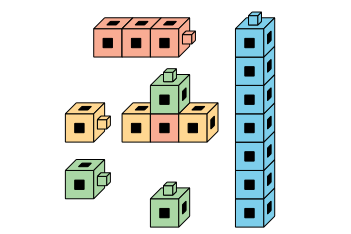
\includegraphics[width=\linewidth, center]{external/svg-source/tikz-file-147993.pdf}
\end{image}%
\end{exploration}%
\end{subsubsectionptx}
%
%
\typeout{************************************************}
\typeout{Subsubsección  Actividad 1}
\typeout{************************************************}
%
% \begin{subsubsectionptx}{Subsubsección}{Actividad 1}{}{Actividad 1}{}{}{lec-explorarCubosEncajables-act1}
% \begin{activity}{Actividad}{Conozcamos\\“Cubos encajables: Explora”.}{act-conozcamos-CubosEncajables-Explora}%
% ¡A explorar!%
% \end{activity}%
% \end{subsubsectionptx}
\end{subsectionptx}
%
%
\typeout{************************************************}
\typeout{Subsección  Lección 2 -~Exploremos las fichas geométricas}
\typeout{************************************************}
%
\begin{subsectionptx}{Subsección}{{\normalsize Lección 2\\[-0.05cm]}Exploremos las fichas geométricas}{}{Lección 2}{}{}{lec-exploremosFichasGeometricas}
\begin{introduction}{}%
Exploremos las fichas geométricas.%
\end{introduction}%
%
%
\typeout{************************************************}
\typeout{Subsubsección  Calentamiento}
\typeout{************************************************}
%
\begin{subsubsectionptx}{Subsubsección}{Calentamiento}{}{Calentamiento}{}{}{lec-exploremosFichasGeometricas-warm}
\begin{exploration}{Calentamiento}{Observa y pregúntate: Fichas geométricas.}{warm-observa-fichasGeometricas}%
¿Qué observas?\\
 ¿Qué te preguntas?%
\begin{image}{0}{1}{0}{}%
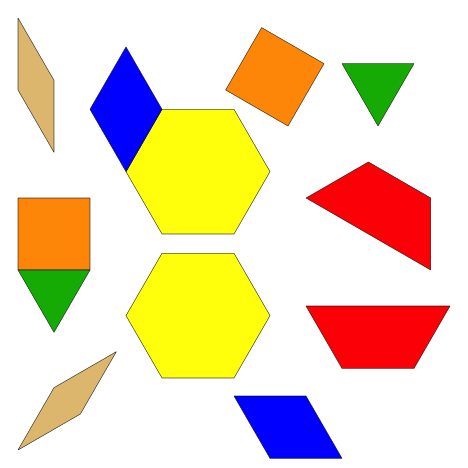
\includegraphics[max width=0.65\linewidth, center]{external/svg-source/tikz-file-148141.pdf}
\end{image}%
\end{exploration}%
\end{subsubsectionptx}
%
%
\typeout{************************************************}
\typeout{Subsubsección  Actividad 1}
\typeout{************************************************}
%
% \begin{subsubsectionptx}{Subsubsección}{Actividad 1}{}{Actividad 1}{}{}{lec-exploremosFichasGeometricas-act1}
% \begin{activity}{Actividad}{Conozcamos\\"Fichas geométricas: Explora".}{act-conozcamos-fichasGeometricas-explora}%
% ¡A explorar!%
% \end{activity}%
% \end{subsubsectionptx}
\end{subsectionptx}
%
%
\typeout{************************************************}
\typeout{Subsección  Lección 3 -~Exploremos las fichas de dos colores y los tableros de 5}
\typeout{************************************************}
%
\begin{subsectionptx}{Subsección}{{\normalsize Lección 3\\[-0.05cm]}Exploremos las fichas de dos colores y los tableros de 5}{}{Lección 3}{}{}{lec-exploremosFichasDosColoresYTableros5}
% \begin{introduction}{}%
% Exploremos las fichas de dos colores y los tableros de 5.%
% \end{introduction}%
%
%
\typeout{************************************************}
\typeout{Subsubsección  Calentamiento}
\typeout{************************************************}
%
\begin{subsubsectionptx}{Subsubsección}{Calentamiento}{}{Calentamiento}{}{}{lec-exploremosFichasDosColoresYTableros5-warm}
\begin{exploration}{Calentamiento}{Observa y pregúntate: fichas y tableros de 5.}{warm-observa-fichasYTableros5}%
¿Qué observas?\\
 ¿Qué te preguntas?%
\begin{sidebyside}{2}{0.05}{0.05}{0.1}%
\begin{sbspanel}{0.4}%

\includegraphics[max width=\linewidth, center]{external/svg-source/tikz-file-147345.pdf}
\end{sbspanel}%
\begin{sbspanel}{0.4}%
\includegraphics[max width=\linewidth, center]{external/png-source/K.1.A Beta Student Workbook.RedYellowChips_withShadow.png}
\end{sbspanel}%
\end{sidebyside}%
\begin{sidebyside}{2}{0.05}{0.05}{0.1}%
\begin{sbspanel}{0.4}%
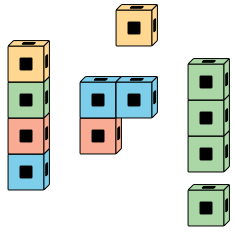
\includegraphics[max width=\linewidth, center]{external/svg-source/tikz-file-128850.pdf}
\end{sbspanel}%
\begin{sbspanel}{0.4}%
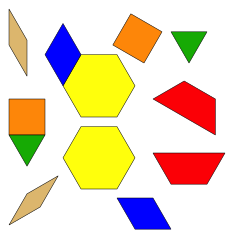
\includegraphics[max width=\linewidth, center]{external/svg-source/tikz-file-147344.pdf}
\end{sbspanel}%
\end{sidebyside}%
\end{exploration}%
\end{subsubsectionptx}
%
%
\typeout{************************************************}
\typeout{Subsubsección  Actividad 1}
\typeout{************************************************}
%
% \begin{subsubsectionptx}{Subsubsección}{Actividad 1}{}{Actividad 1}{}{}{lec-exploremosFichasDosColoresYTableros5-act1}
% \begin{activity}{Actividad}{Exploremos fichas y tableros de 5.}{act-exploremosFichasYTableros5}%
% \begin{image}{0}{1}{0}{}%
% 
\includegraphics[max width=\linewidth, center]{external/svg-source/tikz-file-148144.pdf}
% \end{image}%
% \end{activity}%
% \end{subsubsectionptx}
\end{subsectionptx}
%
%
\typeout{************************************************}
\typeout{Subsección  Lección 4 -~Exploremos los bloques sólidos geométricos}
\typeout{************************************************}
%
\begin{subsectionptx}{Subsección}{{\normalsize Lección 4\\[-0.05cm]}Exploremos los bloques sólidos geométricos}{}{Lección 4}{}{}{lec-exploremosBloquesSolidosGeom}
% \begin{introduction}{}%
% Exploremos los bloques sólidos geométricos.%
% \end{introduction}%
%
%
\typeout{************************************************}
\typeout{Subsubsección  Calentamiento}
\typeout{************************************************}
%
\begin{subsubsectionptx}{Subsubsección}{Calentamiento}{}{Calentamiento}{}{}{lec-exploremosBloquesSolidosGeom-warm}
\begin{exploration}{Calentamiento}{Observa y pregúntate: Bloques sólidos geométricos.}{warm-observa-bloquesSolidosGeom}%
¿Qué observas?\\
 ¿Qué te preguntas?%
\begin{image}{0.0}{1}{0.0}{}%
\includegraphics[max width=\linewidth, center]{external/png-source/K.1.A Beta Student Workbook.Geoblocks.png}
\end{image}%
\end{exploration}%
\end{subsubsectionptx}
%
%
\typeout{************************************************}
\typeout{Subsubsección  Actividad 1}
\typeout{************************************************}
%
% \begin{subsubsectionptx}{Subsubsección}{Actividad 1}{}{Actividad 1}{}{}{lec-exploremosBloquesSolidosGeom-act1}
% \begin{activity}{Actividad}{Conozcamos\\``Bloques sólidos geométricos: Explora''.}{act-conozcamos-bloquesSolidosGeom-explora}%
% ¡Exploremos con los bloques!%
% \end{activity}%
% \end{subsubsectionptx}
%
%
\typeout{************************************************}
\typeout{Subsubsección  Actividad 2}
\typeout{************************************************}
%
% \clearpage
\begin{subsubsectionptx}{Subsubsección}{Actividad 2}{}{Actividad 2}{}{}{lec-exploremosBloquesSolidosGeom-act2}
\begin{activity}{Actividad}{Conozcamos\\“Bloques sólidos geométricos: Construye lo que ves”.}{act-conozcamos-bloquesSolidosGeom-construyeVes}%
Usa bloques para construir una casa.%
\begin{image}{0}{1}{0}{}%
\includegraphics[width=\linewidth, center]{external/png-source/house.png}
\end{image}%
\end{activity}%
\end{subsubsectionptx}
\end{subsectionptx}
%
%
\typeout{************************************************}
\typeout{Subsección  Lección 5 -~Exploremos nuestras herramientas matemáticas}
\typeout{************************************************}
%
\begin{subsectionptx}{Subsección}{{\normalsize Lección 5\\[-0.05cm]}Exploremos nuestras herramientas matemáticas}{}{Lección 5}{}{}{lec-exploremosHerramientasMate}
\begin{introduction}{}%
Exploremos nuestras herramientas matemáticas.%
\end{introduction}%
%
%
\typeout{************************************************}
\typeout{Subsubsección  Calentamiento}
\typeout{************************************************}
%
\begin{subsubsectionptx}{Subsubsección}{Calentamiento}{}{Calentamiento}{}{}{lec-exploremosHerramientasMate-warm}
\begin{exploration}{Calentamiento}{Observa y pregúntate: Usa herramientas distintas.}{warm-observa-herramientasDistintas}%
¿Qué observas?\\
 ¿Qué te preguntas?%
\begin{sidebyside}{2}{0.05}{0.05}{0.1}%
\begin{sbspanel}{0.4}%
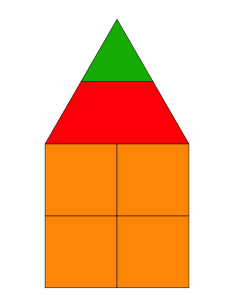
\includegraphics[max width=\linewidth, center]{external/svg-source/tikz-file-148145.pdf}
\end{sbspanel}%
\begin{sbspanel}{0.4}%
\includegraphics[max width=\linewidth, center]{external/png-source/K.1.A Beta Student Workbook.Woodhouse_withShadow.png}
\par
\includegraphics[max width=\linewidth, center]{external/png-source/5.1.A2.House_withShadow.png}
\end{sbspanel}%
\end{sidebyside}%
\end{exploration}%
\end{subsubsectionptx}
%
%
\typeout{************************************************}
\typeout{Subsubsección  Actividad 1}
\typeout{************************************************}
%
% \begin{multicols}{2}
\begin{subsubsectionptx}{Subsubsección}{Actividad 1}{}{Actividad 1}{}{}{lec-exploremosHerramientasMate-act1}
\begin{activity}{Actividad}{Conozcamos\\“Cubos encajables: Construye lo que ves”.}{act-conozcamos-construyeLoQueVes}%
\begin{image}{0}{1}{0}{}%
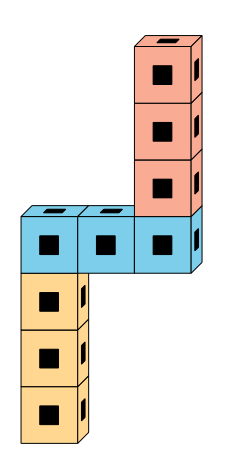
\includegraphics[ width=0.26\linewidth, center]{external/svg-source/tikz-file-148146.pdf}
\end{image}%
\end{activity}%
\end{subsubsectionptx}
%
%
\typeout{************************************************}
\typeout{Subsubsección  Actividad 2}
\typeout{************************************************}
%
\begin{subsubsectionptx}{Subsubsección}{Actividad 2}{}{Actividad 2}{}{}{lec-exploremosHerramientasMate-act2}
\begin{activity}{Actividad}{Conozcamos\\“Fichas geométricas: Rompecabezas”.}{act-conozcamos-fichasGeometricas-rompecabezas}%
\begin{image}{0}{1}{0}{}%
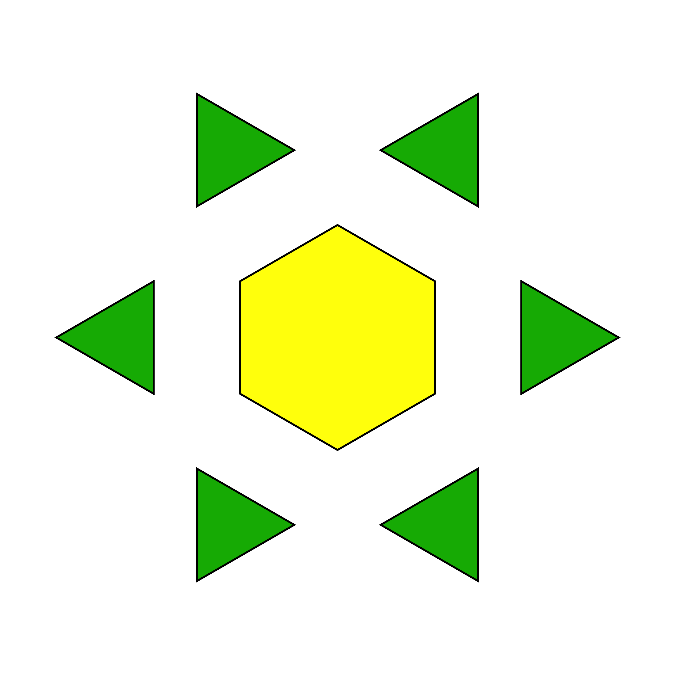
\includegraphics[width=0.5\linewidth, center]{external/svg-source/tikz-file-148147.pdf}
\end{image}%
\end{activity}%
\end{subsubsectionptx}
% \end{multicols}
%
%
\typeout{************************************************}
\typeout{Subsubsección  Actividad 3}
\typeout{************************************************}
%
\clearpage
\begin{subsubsectionptx}{Subsubsección}{Actividad 3}{}{Actividad 3}{}{}{lec-exploremosHerramientasMate-act3}
\begin{activity}{Actividad}{Centros: Momento de escoger.}{act-centros-escoger1}%
Escoge un centro.%
\begin{sidebyside}{2}{0.05}{0.05}{0.1}%
\begin{sbspanel}{0.5}[center]%
Bloques sólidos geométricos%
\end{sbspanel}%
\begin{sbspanel}{0.3}[center]%
\includegraphics[max width=\linewidth, center]{external/png-source/K.1.A Beta Student Workbook.Geoblocks.png}
\end{sbspanel}%
\end{sidebyside}%
\begin{sidebyside}{2}{0.05}{0.05}{0.1}%
\begin{sbspanel}{0.5}[center]%
Cubos encajables%
\end{sbspanel}%
\begin{sbspanel}{0.3}[center]%
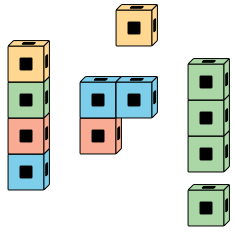
\includegraphics[max width=\linewidth, center]{external/svg-source/tikz-file-128850.pdf}
\end{sbspanel}%
\end{sidebyside}%
\begin{sidebyside}{2}{0.05}{0.05}{0.1}%
\begin{sbspanel}{0.5}[center]%
Fichas geométricas%
\end{sbspanel}%
\begin{sbspanel}{0.3}[center]%
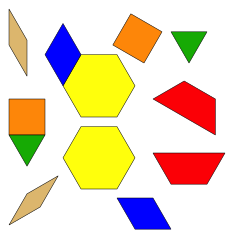
\includegraphics[max width=\linewidth, center]{external/svg-source/tikz-file-147344.pdf}
\end{sbspanel}%
\end{sidebyside}%
\end{activity}%
\end{subsubsectionptx}
\end{subsectionptx}
%
%
\typeout{************************************************}
\typeout{Referencias  Resumen de la sección}
\typeout{************************************************}
%
\begin{references-subsection}{Referencias}{Resumen de la sección}{}{Resumen sección}{}{}{gra0-uni1-secA-resumen}
Exploramos muchas herramientas matemáticas.%
\begin{sidebyside}{2}{0.05}{0.05}{0.1}%
\begin{sbspanel}{0.4}%
Cubos Encajables%
\par
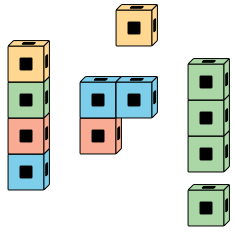
\includegraphics[max width=\linewidth, center]{external/svg-source/tikz-file-128850.pdf}
\end{sbspanel}%
\begin{sbspanel}{0.4}%
Fichas Geométricas%
\par
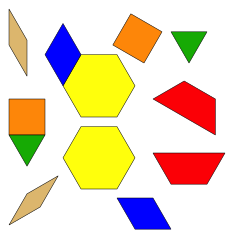
\includegraphics[max width=\linewidth, center]{external/svg-source/tikz-file-147344.pdf}
\end{sbspanel}%
\end{sidebyside}%
\begin{sidebyside}{2}{0.05}{0.05}{0.1}%
\begin{sbspanel}{0.4}%
Bloques sólidos geométricos%
\par
\includegraphics[max width=\linewidth, center]{external/png-source/K.1.A Beta Student Workbook.Geoblocks.png}
\end{sbspanel}%
\begin{sbspanel}{0.4}%
Fichas de dos colores%
\par
\includegraphics[max width=\linewidth, center]{external/png-source/K.1.A Beta Student Workbook.RedYellowChips_withShadow.png}
\end{sbspanel}%
\end{sidebyside}%
\begin{sidebyside}{2}{0.05}{0.05}{0.1}%
\begin{sbspanel}{0.4}%
Tableros de 5%
\par

\includegraphics[max width=\linewidth, center]{external/svg-source/tikz-file-148144.pdf}
\end{sbspanel}%
\begin{sbspanel}{0.4}%
%
\end{sbspanel}%
\end{sidebyside}%
\end{references-subsection}
\end{sectionptx}
%
%
\typeout{************************************************}
\typeout{Sección  Sección B -~Reconozcamos cantidades}
\typeout{************************************************}
%
\begin{sectionptx}{Sección}{{\Large Sección B\\}Reconozcamos cantidades}{}{Sección B -~Reconozcamos cantidades}{}{}{gra0-uni1-secB}
%
%
\typeout{************************************************}
\typeout{Subsección  Lección 6 -~Busquemos grupos pequeños}
\typeout{************************************************}
%
\begin{subsectionptx}{Subsección}{{\normalsize Lección 6\\[-0.05cm]}Busquemos grupos pequeños}{}{Lección 6}{}{}{lec-busquemosGruposMasPequenos}
\begin{introduction}{}%
Busquemos grupos pequeños de objetos.%
\end{introduction}%
%
%
\typeout{************************************************}
\typeout{Subsubsección  Calentamiento}
\typeout{************************************************}
%
\begin{subsubsectionptx}{Subsubsección}{Calentamiento}{}{Calentamiento}{}{}{lec-busquemosGruposMasPequenos-warm}
\begin{exploration}{Calentamiento}{Actuémoslo: Introducción.}{warm-actuemoslo-intro}%
\begin{image}{0.1}{0.8}{0.1}{}%
\includegraphics[max width=\linewidth, center]{external/png-source/3 ducks.png}
\end{image}%
\par
\vspace*{2ex}
3 patitos muy lejos de aquí\\
 a la colina salieron a pasear.\\
 Mamá pata dijo: “Cuac, cuac, cuac”.\\
 Después 3 patitos vio regresar.%
\end{exploration}%
\end{subsubsectionptx}
%
%
\typeout{************************************************}
\typeout{Subsubsección  Actividad 1}
\typeout{************************************************}
%
% \clearpage
\begin{subsubsectionptx}{Subsubsección}{Actividad 1}{}{Actividad 1}{}{}{lec-busquemosGruposMasPequenos-act1}
\begin{activity}{Actividad}{Cuántos ves: Introducción.}{act-cuantosVes-intro}%
\begin{minipage}{0.6\linewidth}
¿Cuántos ves?\\
 ¿Cómo lo sabes?, ¿qué ves?%
\end{minipage}
\hfill
\begin{minipage}{0.3\linewidth}
\begin{image}{0}{1}{0}{}%

\includegraphics[max width=\linewidth, center]{external/svg-source/tikz-file-148150.pdf}
\end{image}%
\end{minipage}
% \end{multicols}
\end{activity}%
\end{subsubsectionptx}
%
%
\typeout{************************************************}
\typeout{Subsubsección  Actividad 2}
\typeout{************************************************}
%
% \clearpage
% \begin{subsubsectionptx}{Subsubsección}{Actividad 2}{}{Actividad 2}{}{}{lec-busquemosGruposMasPequenos-act2}
% \begin{activity}{Actividad}{Conozcamos\\“Libros de imágenes: Explora”.}{act-conozcamos-librosDeImagenes-explora}%
% Busquen grupos de cosas en su libro.%
% \end{activity}%
% \end{subsubsectionptx}
%
%
\typeout{************************************************}
\typeout{Subsubsección  Actividad 3}
\typeout{************************************************}
%
\clearpage
\begin{subsubsectionptx}{Subsubsección}{Actividad 3}{}{Actividad 3}{}{}{lec-busquemosGruposMasPequenos-act3}
\begin{activity}{Actividad}{Centros: Momento de escoger.}{act-centros-escoger2}%
\begin{sidebyside}{2}{0.025}{0.025}{0.05}%
\begin{sbspanel}{0.45}%
Cubos Encajables%
\par
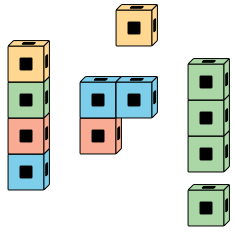
\includegraphics[max width=\linewidth, center]{external/svg-source/tikz-file-128850.pdf}
\end{sbspanel}%
\begin{sbspanel}{0.45}%
Fichas Geométricas%
\par
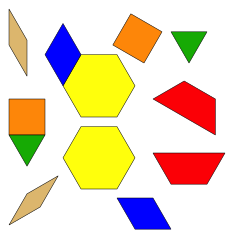
\includegraphics[max width=\linewidth, center]{external/svg-source/tikz-file-147344.pdf}
\end{sbspanel}%
\end{sidebyside}%
\vspace*{1ex minus 0.8ex}
\begin{sidebyside}{2}{0.025}{0.025}{0.05}%
\begin{sbspanel}{0.45}%
Bloques sólidos geométricos%
\par
\includegraphics[max width=\linewidth, center]{external/png-source/K.1.A Beta Student Workbook.Geoblocks.png}
\end{sbspanel}%
\begin{sbspanel}{0.45}%
Libros de imágenes%
\par
\includegraphics[max width=\linewidth, center]{external/png-source/K.1.D Beta Student Workbooks.Books.png}
\end{sbspanel}%
\end{sidebyside}%
\end{activity}%
\end{subsubsectionptx}
\end{subsectionptx}
%
%
\typeout{************************************************}
\typeout{Subsección  Lección 7 -~Juego de búsqueda en el salón de clase}
\typeout{************************************************}
%
\begin{subsectionptx}{Subsección}{{\normalsize Lección 7\\[-0.05cm]}Juego de búsqueda en el salón de clase}{}{Lección 7}{}{}{lec-juegoBusqueda}
\begin{introduction}{}%
Busquemos grupos de objetos en el salón de clase.%
\end{introduction}%
%
%
\typeout{************************************************}
\typeout{Subsubsección  Calentamiento}
\typeout{************************************************}
%
\begin{subsubsectionptx}{Subsubsección}{Calentamiento}{}{Calentamiento}{}{}{lec-juegoBusqueda-warm}
\begin{exploration}{Calentamiento}{¿Cómo lo podemos mostrar?}{warm-comoPodemosMostrar}%
\begin{image}{0.0}{1}{0.0}{}%
\includegraphics[max width=\linewidth, center]{external/png-source/3 ducks.png}
\end{image}%
%
\par
\vspace*{2ex}
3 patitos muy lejos de aqui\\
 a la colina salieron a pasear.\\
 Mamá pata dijo: “Cuac, cuac, cuac”.\\
 Después 3 patitos vio regresar.%
\end{exploration}%
\end{subsubsectionptx}
%
%
\typeout{************************************************}
\typeout{Subsubsección  Actividad 1}
\typeout{************************************************}
%
\clearpage
\begin{subsubsectionptx}{Subsubsección}{Actividad 1}{}{Actividad 1}{}{}{lec-juegoBusqueda-act1}
\begin{activity}{Actividad}{Cuántos ves: Dos imágenes.}{act-cuantosVes-imagenes}%
¿Cuántos ves?\\
 ¿Cómo lo sabes?, ¿qué ves?%
\begin{sidebyside}{2}{0}{0}{0}%
\begin{sbspanel}{0.5}%

\includegraphics[max width=\linewidth, center]{external/svg-source/tikz-file-148152.pdf}
\end{sbspanel}%
\begin{sbspanel}{0.5}%

\includegraphics[max width=\linewidth, center]{external/svg-source/tikz-file-148153.pdf}
\end{sbspanel}%
\end{sidebyside}%
\end{activity}%
\end{subsubsectionptx}
%
%
\typeout{************************************************}
\typeout{Subsubsección  Actividad 2}
\typeout{************************************************}
%
\begin{subsubsectionptx}{Subsubsección}{Actividad 2}{}{Actividad 2}{}{}{lec-juegoBusqueda-act2}
\begin{activity}{Actividad}{Juego de búsqueda en el salón de clase.}{act-juegoBusqueda}%
Busca 3 objetos en nuestro salón.%
\end{activity}%
\end{subsubsectionptx}
%
%
\typeout{************************************************}
\typeout{Subsubsección  Actividad 3}
\typeout{************************************************}
%
\clearpage
\begin{subsubsectionptx}{Subsubsección}{Actividad 3}{}{Actividad 3}{}{}{lec-juegoBusqueda-act3}
\begin{activity}{Actividad}{Centros: Momento de escoger.}{act-centros-escoger3}%
Escoge un centro.%
\begin{sidebyside}{2}{0.025}{0.025}{0.05}%
\begin{sbspanel}{0.45}%
Cubos Encajables%
\par
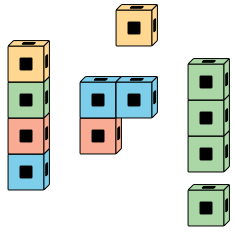
\includegraphics[max width=\linewidth, center]{external/svg-source/tikz-file-128850.pdf}
\end{sbspanel}%
\begin{sbspanel}{0.45}%
Fichas Geométricas%
\par
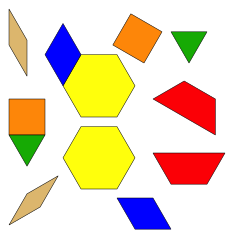
\includegraphics[max width=\linewidth, center]{external/svg-source/tikz-file-147344.pdf}
\end{sbspanel}%
\end{sidebyside}%
\vspace*{1ex minus 0.8ex}
\begin{sidebyside}{2}{0.025}{0.025}{0.05}%
\begin{sbspanel}{0.45}%
Bloques sólidos geométricos%
\par
\includegraphics[max width=\linewidth, center]{external/png-source/K.1.A Beta Student Workbook.Geoblocks.png}
\end{sbspanel}%
\begin{sbspanel}{0.45}%
Libros de imágenes%
\par
\includegraphics[max width=\linewidth, center]{external/png-source/K.1.D Beta Student Workbooks.Books.png}
\end{sbspanel}%
\end{sidebyside}%
\end{activity}%
\end{subsubsectionptx}
\end{subsectionptx}
%
%
\typeout{************************************************}
\typeout{Subsección  Lección 8 -~Grupos diferentes, misma cantidad}
\typeout{************************************************}
%
\begin{subsectionptx}{Subsección}{{\normalsize Lección 8\\[-0.05cm]}Grupos diferentes, misma cantidad}{}{Lección 8}{}{}{lec-gruposDiferentesMismaCantidad}
\begin{introduction}{}%
Encontremos grupos que tengan el mismo número de cosas.%
\end{introduction}%
%
%
\typeout{************************************************}
\typeout{Subsubsección  Calentamiento}
\typeout{************************************************}
%
\begin{subsubsectionptx}{Subsubsección}{Calentamiento}{}{Calentamiento}{}{}{lec-gruposDiferentesMismaCantidad-warm}
\begin{exploration}{Calentamiento}{Actuémoslo: Otra manera.}{warm-actuemoslo-otraManera}%
\begin{image}{0.0}{1}{0.0}{}%
\includegraphics[max width=\linewidth, center]{external/png-source/3 ducks.png}
\end{image}%
%
\par
\vspace*{2ex}
3 patitos muy lejos de aquí\\
 a la colina salieron a pasear.\\
 Mamá pata dijo: “Cuac, cuac, cuac.”\\
 Después 3 patitos vio regresar.%
\end{exploration}%
\end{subsubsectionptx}
%
%
\typeout{************************************************}
\typeout{Subsubsección  Actividad 1}
\typeout{************************************************}
%
\clearpage
\begin{subsubsectionptx}{Subsubsección}{Actividad 1}{}{Actividad 1}{}{}{lec-gruposDiferentesMismaCantidad-act1}
\begin{activity}{Actividad}{Cuántos ves: 1, 2, 3.}{act-cuantosVes-123}%
¿Cuántos ves?\\
 ¿Cómo lo sabes?, ¿qué ves?%
\begin{sidebyside}{3}{0.0416666666666667}{0.0416666666666667}{0.0833333333333333}%
\begin{sbspanel}{0.25}%

\includegraphics[max width=\linewidth, center]{external/svg-source/tikz-file-136322.pdf}
\end{sbspanel}%
\begin{sbspanel}{0.25}%

\includegraphics[max width=\linewidth, center]{external/svg-source/tikz-file-136323.pdf}
\end{sbspanel}%
\begin{sbspanel}{0.25}%

\includegraphics[max width=\linewidth, center]{external/svg-source/tikz-file-136324.pdf}
\end{sbspanel}%
\end{sidebyside}%
\end{activity}%
\end{subsubsectionptx}
%
%
\typeout{************************************************}
\typeout{Subsubsección  Actividad 2}
\typeout{************************************************}
%
\begin{subsubsectionptx}{Subsubsección}{Actividad 2}{}{Actividad 2}{}{}{lec-gruposDiferentesMismaCantidad-act2}
\begin{activity}{Actividad}{Grupos diferentes, misma cantidad.}{act-gruposDiferentesMismaCantidad}%
\begin{image}{0}{1}{0}{}%
\includegraphics[max width=\linewidth, center]{external/png-source/K.1.C Beta Student Workbook.AnimalGroups.png}
\end{image}%
%
\end{activity}%
\end{subsubsectionptx}
%
%
\typeout{************************************************}
\typeout{Subsubsección  Actividad 3}
\typeout{************************************************}
%
\clearpage
\begin{subsubsectionptx}{Subsubsección}{Actividad 3}{}{Actividad 3}{}{}{lec-gruposDiferentesMismaCantidad-act3}
\begin{activity}{Actividad}{Centros: Momento de escoger.}{act-centros-escoger4}%
Escoge un centro.%
\begin{sidebyside}{2}{0.025}{0.025}{0.05}%
\begin{sbspanel}{0.45}%
Cubos Encajables%
\par
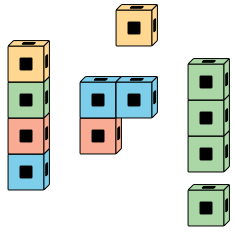
\includegraphics[max width=\linewidth, center]{external/svg-source/tikz-file-128850.pdf}
\end{sbspanel}%
\begin{sbspanel}{0.45}%
Fichas Geométricas%
\par
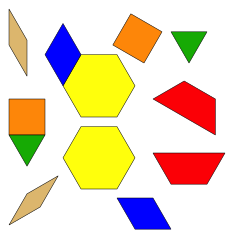
\includegraphics[max width=\linewidth, center]{external/svg-source/tikz-file-147344.pdf}
\end{sbspanel}%
\end{sidebyside}%
\vspace*{1ex minus 0.8ex}
\begin{sidebyside}{2}{0.025}{0.025}{0.05}%
\begin{sbspanel}{0.45}%
Bloques sólidos geométricos%
\par
\includegraphics[max width=\linewidth, center]{external/png-source/K.1.A Beta Student Workbook.Geoblocks.png}
\end{sbspanel}%
\begin{sbspanel}{0.45}%
Libros de imágenes%
\par
\includegraphics[max width=\linewidth, center]{external/png-source/K.1.D Beta Student Workbooks.Books.png}
\end{sbspanel}%
\end{sidebyside}%
\end{activity}%
\end{subsubsectionptx}
\end{subsectionptx}
%
%
\typeout{************************************************}
\typeout{Subsección  Lección 9 -~Hagamos libros de imágenes}
\typeout{************************************************}
%
\begin{subsectionptx}{Subsección}{{\normalsize Lección 9\\[-0.05cm]}Hagamos libros de imágenes}{}{Lección 9}{}{}{lec-hagamosDeLibrosImagenes}
\begin{introduction}{}%
Hagamos libros de imágenes acerca de nuestro salón de clase.%
\end{introduction}%
%
%
\typeout{************************************************}
\typeout{Subsubsección  Calentamiento}
\typeout{************************************************}
%
\begin{subsubsectionptx}{Subsubsección}{Calentamiento}{}{Calentamiento}{}{}{lec-hagamosDeLibrosImagenes-warm}
\begin{exploration}{Calentamiento}{Actuémoslo: La historia cambia.}{warm-actuemoslo-laHistoriaCambia}%
\begin{image}{0.0}{1}{0.0}{}%
\includegraphics[max width=\linewidth, center]{external/png-source/3 ducks.png}
\end{image}%
%
\par
\vspace*{2ex}
3 patitos muy lejos de aquí\\
 a la colina salieron a pasear.\\
 Mamá pata dijo: “Cuac, cuac, cuac.”\\
 Después 3 patitos vio regresar.%
\par
3 patitos muy lejos de aquí\\
 a la colina salieron a pasear.\\
 Mamá pata dijo: “Cuac, cuac, cuac.”\\
 Después 2 patitos vio regresar.%
\end{exploration}%
\end{subsubsectionptx}
%
%
\typeout{************************************************}
\typeout{Subsubsección  Actividad 1}
\typeout{************************************************}
%
\clearpage
\begin{subsubsectionptx}{Subsubsección}{Actividad 1}{}{Actividad 1}{}{}{lec-hagamosDeLibrosImagenes-act1}
\begin{activity}{Actividad}{Cuántos ves: ¿Qué observas?}{act-cuantosVes-queObservas}%
¿Cuántos ves?\\
 ¿Cómo lo sabes?, ¿qué ves?%
\begin{sidebyside}{2}{0}{0}{0}%
\begin{sbspanel}{0.5}%

\includegraphics[max width=\linewidth, center]{external/svg-source/tikz-file-148154.pdf}
\end{sbspanel}%
\begin{sbspanel}{0.5}%
\includegraphics[max width=\linewidth, center]{external/svg-source/tikz-file-147348.pdf}
\end{sbspanel}%
\end{sidebyside}%
\end{activity}%
\end{subsubsectionptx}
%
%
\typeout{************************************************}
\typeout{Subsubsección  Actividad 2}
\typeout{************************************************}
%
\begin{subsubsectionptx}{Subsubsección}{Actividad 2}{}{Actividad 2}{}{}{lec-hagamosDeLibrosImagenes-act2}
\begin{activity}{Actividad}{Conozcamos\\“Libros de imágenes: Crea”.}{act-conozcamos-librosDeImagenes-crea}%
Dibuja cosas de nuestro salón de las que haya dos.%
\begin{sidebyside}{2}{0.3}{0.3}{0}%
\begin{sbspanel}{0.2}%

\includegraphics[max width=\linewidth, center]{external/svg-source/tikz-file-148155.pdf}
\end{sbspanel}%
\begin{sbspanel}{0.2}%

\includegraphics[max width=\linewidth, center]{external/svg-source/tikz-file-148154.pdf}
\end{sbspanel}%
\end{sidebyside}%
\end{activity}%
\end{subsubsectionptx}
%
%
\typeout{************************************************}
\typeout{Subsubsección  Actividad 3}
\typeout{************************************************}
%
\clearpage
\begin{subsubsectionptx}{Subsubsección}{Actividad 3}{}{Actividad 3}{}{}{lec-hagamosDeLibrosImagenes-act3}
\begin{activity}{Actividad}{Centros: Momento de escoger.}{act-centros-escoger5}%
Escoge un centro.%
\begin{sidebyside}{2}{0.025}{0.025}{0.05}%
\begin{sbspanel}{0.45}%
Cubos Encajables%
\par
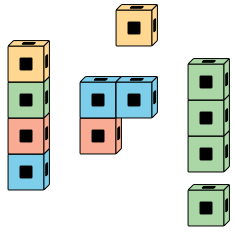
\includegraphics[max width=\linewidth, center]{external/svg-source/tikz-file-128850.pdf}
\end{sbspanel}%
\begin{sbspanel}{0.45}%
Fichas Geométricas%
\par
\includegraphics[max width=\linewidth, center]{external/svg-source/tikz-file-147344.pdf}
\end{sbspanel}%
\end{sidebyside}%
\vspace*{1ex minus 0.8ex}
\begin{sidebyside}{2}{0.025}{0.025}{0.05}%
\begin{sbspanel}{0.45}%
Bloques sólidos geométricos%
\par
\includegraphics[max width=\linewidth, center]{external/png-source/K.1.A Beta Student Workbook.Geoblocks.png}
\end{sbspanel}%
\begin{sbspanel}{0.45}%
Libros de imágenes%
\par
\includegraphics[max width=\linewidth, center]{external/png-source/K.1.D Beta Student Workbooks.Books.png}
\end{sbspanel}%
\end{sidebyside}%
\end{activity}%
\end{subsubsectionptx}
\end{subsectionptx}
%
%
\typeout{************************************************}
\typeout{Referencias  Resumen de la lección}
\typeout{************************************************}
%
\begin{references-subsection}{Referencias}{Resumen de la lección}{}{Resumen sección}{}{}{gra0-uni1-secB-resumen}
En esta sección, observamos las matemáticas que hay en nuestro mundo.%
\par
Encontramos grupos de cosas en nuestro salón de clase y en libros.
 Usamos nuestros dedos y dijimos números para mostrar cuántas cosas había.%
\par
\begin{sidebyside}{2}{0.1}{0.1}{0.2}%
\begin{sbspanel}{0.5}%
\includegraphics[max width=\linewidth, center]{external/png-source/2-windows.png}
\end{sbspanel}%
\begin{sbspanel}{0.1}%
\includegraphics[max width=\linewidth, center]{external/svg-source/tikz-file-136325.pdf}
\end{sbspanel}%
\end{sidebyside}%
%
\par
Encontramos grupos que tienen el mismo número de cosas.%
\par
Hay 2 ventanas y 2 mesas.%
\begin{sidebyside}{2}{0.025}{0.025}{0.05}%
\begin{sbspanel}{0.5}%
\includegraphics[max width=\linewidth, center]{external/png-source/2-windows.png}
\end{sbspanel}%
\begin{sbspanel}{0.4}%
\includegraphics[max width=\linewidth, center]{external/png-source/2-tables.png}
\end{sbspanel}%
\end{sidebyside}%
\par
Hay 3 estrellas y 3 balones de fútbol.%
\begin{sidebyside}{2}{0.1}{0.1}{0.2}%
\begin{sbspanel}{0.3}%
\includegraphics[max width=\linewidth, center]{external/png-source/K.1.C11.BLM.F.png}
\end{sbspanel}%
\begin{sbspanel}{0.3}%
\includegraphics[max width=\linewidth, center]{external/png-source/K.1.C11.BLM.H.png}
\end{sbspanel}%
\end{sidebyside}%
\par
Se ven diferentes, pero ambos grupos tienen 3 cosas.%
\par
Creamos nuestros propios libros para mostrar grupos que tienen el mismo número  de cosas en nuestro salón.%
\begin{image}{0.2}{0.6}{0.2}{}%
\includegraphics[max width=\linewidth, center]{external/png-source/BLM picture books-2.png}
\end{image}%
\end{references-subsection}
\end{sectionptx}
%
%
\typeout{************************************************}
\typeout{Sección  Sección C -~¿Hay suficientes?}
\typeout{************************************************}
%
\begin{sectionptx}{Sección}{{\Large Sección C\\}¿Hay suficientes?}{}{Sección C -~¿Hay suficientes?}{}{}{gra0-uni1-secC}
%
%
\typeout{************************************************}
\typeout{Subsección  Lección 10 -~Cuántos ves: Construyamos sobre lo aprendido}
\typeout{************************************************}
%
\begin{subsectionptx}{Subsección}{{\normalsize Lección 10\\[-0.05cm]}Cuántos ves: Construyamos sobre lo aprendido}{}{Lección 10}{}{}{lec-cuantosVesConstruyamosSobreLoAprendido}
\begin{introduction}{}%
Averigüemos si hay suficientes materiales para todos.%
\end{introduction}%
%
%
\typeout{************************************************}
\typeout{Subsubsección  Calentamiento}
\typeout{************************************************}
%
\begin{subsubsectionptx}{Subsubsección}{Calentamiento}{}{Calentamiento}{}{}{lec-cuantosVesConstruyamosSobreLoAprendido-warm}
\begin{exploration}{Calentamiento}{Cuántos ves: Construyamos sobre lo aprendido.}{warm-cuantosVes-construyamosSobreLoAprendido}%
¿Cuántos ves?\\
 Cómo lo sabes?, ¿qué ves?%
\begin{sidebyside}{2}{0}{0}{0}%
\begin{sbspanel}{0.5}%
\includegraphics[max width=\linewidth, center]{external/svg-source/tikz-file-136323.pdf}
\end{sbspanel}%
\begin{sbspanel}{0.5}%
\includegraphics[max width=\linewidth, center]{external/svg-source/tikz-file-147346.pdf}
\end{sbspanel}%
\end{sidebyside}%
\end{exploration}%
\end{subsubsectionptx}
%
%
\typeout{************************************************}
\typeout{Subsubsección  Actividad 1}
\typeout{************************************************}
\clearpage
\begin{subsubsectionptx}{Subsubsección}{Actividad 1}{}{Actividad 1}{}{}{lec-cuantosVesConstruyamosSobreLoAprendido-act1}
\begin{activity}{Actividad}{Actuémoslo: Cuatro ranitas manchadas (parte 1).}{act-actuemoslo-cuatroRanitas}%
\begin{image}{0.275}{0.45}{0.275}{}%
\includegraphics[max width=\linewidth, center]{external/png-source/RANA-VERDE.png}
\end{image}%
%
\par
\small
\vspace{2ex}
4 ranitas manchadas se sentaron en un tronco manchado\\
 a comer los más deliciosos bichos. ¡Yum! ¡Yum!\\
 1 saltó al lago, que estaba agradable y fresco.\\
 Ahora hay 3 ranitas verdes manchadas. ¡Glub! ¡Glub!%
\end{activity}%
\end{subsubsectionptx}
%
%
\typeout{************************************************}
\typeout{Subsubsección  Actividad 2}
\typeout{************************************************}
%
% \begin{subsubsectionptx}{Subsubsección}{Actividad 2}{}{Actividad 2}{}{}{lec-cuantosVesConstruyamosSobreLoAprendido-act2}
% \begin{activity}{Actividad}{¿Hay suficientes?}{act-haySuficientes}%
% ¿Hay suficientes?%
% \end{activity}%
% \end{subsubsectionptx}
%
%
\typeout{************************************************}
\typeout{Subsubsección  Actividad 3}
\typeout{************************************************}
%
\clearpage
\begin{subsubsectionptx}{Subsubsección}{Actividad 3}{}{Actividad 3}{}{}{lec-cuantosVesConstruyamosSobreLoAprendido-act3}
\begin{activity}{Actividad}{Centros: Momento de escoger.}{act-centros-escoger6}%
Escoge un centro.%
\begin{sidebyside}{2}{0.025}{0.025}{0.05}%
\begin{sbspanel}{0.45}%
Cubos Encajables%
\par
\includegraphics[max width=\linewidth, center]{external/svg-source/tikz-file-128850.pdf}
\end{sbspanel}%
\begin{sbspanel}{0.45}%
Fichas Geométricas%
\par
\includegraphics[max width=\linewidth, center]{external/svg-source/tikz-file-147344.pdf}
\end{sbspanel}%
\end{sidebyside}%
\vspace*{1ex minus 0.8ex}
\begin{sidebyside}{2}{0.025}{0.025}{0.05}%
\begin{sbspanel}{0.45}%
Bloques sólidos geométricos%
\par
\includegraphics[max width=\linewidth, center]{external/png-source/K.1.A Beta Student Workbook.Geoblocks.png}
\end{sbspanel}%
\begin{sbspanel}{0.45}%
Libros de imágenes%
\par
\includegraphics[max width=\linewidth, center]{external/png-source/K.1.D Beta Student Workbooks.Books.png}
\end{sbspanel}%
\end{sidebyside}%
\end{activity}%
\end{subsubsectionptx}
\end{subsectionptx}
%
%
\typeout{************************************************}
\typeout{Subsección  Lección 11 -~Consigamos suficientes}
\typeout{************************************************}
%
\begin{subsectionptx}{Subsección}{{\normalsize Lección 11\\[-0.05cm]}Consigamos suficientes}{}{Lección 11}{}{}{lec-consigamosSuficientes}
\begin{introduction}{}%
Consigamos suficientes lápices para todos.%
\end{introduction}%
%
%
\typeout{************************************************}
\typeout{Subsubsección  Calentamiento}
\typeout{************************************************}
%
\begin{subsubsectionptx}{Subsubsección}{Calentamiento}{}{Calentamiento}{}{}{lec-consigamosSuficientes-warm}
\begin{exploration}{Calentamiento}{Cuántos ves: En un instante.}{warm-cuantosVes-enUnInstante}%
¿Cuántos ves?\\
 ¿Cómo lo sabes?, ¿qué ves?%
\begin{sidebyside}{2}{0}{0}{0}%
\begin{sbspanel}{0.5}%
\includegraphics[max width=\linewidth, center]{external/svg-source/tikz-file-148153.pdf}
\end{sbspanel}%
\begin{sbspanel}{0.5}%
\includegraphics[max width=\linewidth, center]{external/svg-source/tikz-file-136326.pdf}
\end{sbspanel}%
\end{sidebyside}%
\end{exploration}%
\end{subsubsectionptx}
%
%
\typeout{************************************************}
\typeout{Subsubsección  Actividad 1}
\typeout{************************************************}
%
\clearpage
\begin{subsubsectionptx}{Subsubsección}{Actividad 1}{}{Actividad 1}{}{}{lec-consigamosSuficientes-act1}
\begin{activity}{Actividad}{Actuémoslo: Cuatro ranitas manchadas (parte 2).}{act-actuemoslo-cuatroRanitasParte2}%
\begin{image}{0.275}{0.45}{0.275}{}%
\includegraphics[max width=\linewidth, center]{external/png-source/RANA-VERDE.png}
\end{image}%
%
\par
\small
\vspace{2ex}
4 ranitas manchadas se sentaron en un tronco manchado\\
 a comer los más deliciosos bichos. ¡Yum! ¡Yum!\\
 1 saltó al lago, que estaba agradable y fresco.\\
 Ahora hay 3 ranitas verdes manchadas. ¡Glub! ¡Glub!%
\end{activity}%
\end{subsubsectionptx}
%
%
\typeout{************************************************}
\typeout{Subsubsección  Actividad 2}
\typeout{************************************************}
%
\begin{subsubsectionptx}{Subsubsección}{Actividad 2}{}{Actividad 2}{}{}{lec-consigamosSuficientes-act2}
\begin{activity}{Actividad}{Consigamos suficientes.}{act-consigamosSuficientes}%
\begin{image}{0.0}{1}{0.0}{}%
\includegraphics[max width=\linewidth, center]{external/png-source/K.1 Revisions.StudentFacesInARow.png}
\end{image}%
\end{activity}%
\end{subsubsectionptx}
%
%
\typeout{************************************************}
\typeout{Subsubsección  Actividad 3}
\typeout{************************************************}
%
\clearpage
\begin{subsubsectionptx}{Subsubsección}{Actividad 3}{}{Actividad 3}{}{}{lec-consigamosSuficientes-act3}
\begin{activity}{Actividad}{Centros: Momento de escoger.}{act-centros-escoger7}%
Escoge un centro.%
\begin{sidebyside}{2}{0.025}{0.025}{0.05}%
\begin{sbspanel}{0.45}%
Cubos Encajables%
\par
\includegraphics[max width=\linewidth, center]{external/svg-source/tikz-file-128850.pdf}
\end{sbspanel}%
\begin{sbspanel}{0.45}%
Fichas Geométricas%
\par
\includegraphics[max width=\linewidth, center]{external/svg-source/tikz-file-147344.pdf}
\end{sbspanel}%
\end{sidebyside}%
\vspace*{1ex minus 0.8ex}
\begin{sidebyside}{2}{0.025}{0.025}{0.05}%
\begin{sbspanel}{0.45}%
Bloques sólidos geométricos%
\par
\includegraphics[max width=\linewidth, center]{external/png-source/K.1.A Beta Student Workbook.Geoblocks.png}
\end{sbspanel}%
\begin{sbspanel}{0.45}%
Libros de imágenes%
\par
\includegraphics[max width=\linewidth, center]{external/png-source/K.1.D Beta Student Workbooks.Books.png}
\end{sbspanel}%
\end{sidebyside}%
\end{activity}%
\end{subsubsectionptx}
\end{subsectionptx}
%
%
\typeout{************************************************}
\typeout{Referencias  Resumen de la sección}
\typeout{************************************************}
%
\begin{references-subsection}{Referencias}{Resumen de la sección}{}{Resumen sección}{}{}{gra0-uni1-secC-resumen}
En esta sección, desciframos si había suficientes lápices para cada uno en nuestro grupo.%
\begin{image}{0}{1}{0}{}%
\includegraphics[max width=\linewidth, center]{external/png-source/K.1.C Beta Student Workbook.4Kids4Pencils.png}
\end{image}%
Emparejamos cada lápiz con una persona.%
\par
También conseguimos suficientes lápices para que cada persona pudiera tener uno.%
\end{references-subsection}
\end{sectionptx}
%
%
\typeout{************************************************}
\typeout{Sección  Sección D -~Contemos colecciones}
\typeout{************************************************}
%
\begin{sectionptx}{Sección}{{\Large Sección D\\}Contemos colecciones}{}{Sección D -~Contemos colecciones}{}{}{gra0-uni1-secD}
%
%
\typeout{************************************************}
\typeout{Subsección  Lección 12 -~¿Cuántos hay? (Parte 1)}
\typeout{************************************************}
%
\begin{subsectionptx}{Subsección}{{\normalsize Lección 12\\[-0.05cm]}¿Cuántos hay? (Parte 1)}{}{Lección 12}{}{}{lec-cuantosHayParte1}
\begin{introduction}{}%
Contemos colecciones de objetos%
\end{introduction}%
%
%
\typeout{************************************************}
\typeout{Subsubsección  Calentamiento}
\typeout{************************************************}
%
% \begin{subsubsectionptx}{Subsubsección}{Calentamiento}{}{Calentamiento}{}{}{lec-cuantosHayParte1-warm}
% \begin{exploration}{Calentamiento}{Preguntas sobre nosotros:\\¿Cuántos estamos hoy aquí?}{warm-preguntasNosotros-cuantosEstamos}%
% ¿Cuántos estamos hoy aquí?%
% \end{exploration}%
% \end{subsubsectionptx}
%
%
\typeout{************************************************}
\typeout{Subsubsección  Actividad 1}
\typeout{************************************************}
%
% \begin{subsubsectionptx}{Subsubsección}{Actividad 1}{}{Actividad 1}{}{}{lec-cuantosHayParte1-act1}
% \begin{activity}{Actividad}{Contemos colecciones.}{act-contemosColecciones}%
% ¿Cuántos objetos hay en la colección?%
% \end{activity}%
% \end{subsubsectionptx}
%
%
\typeout{************************************************}
\typeout{Subsubsección  Actividad 2}
\typeout{************************************************}
%
% \begin{subsubsectionptx}{Subsubsección}{Actividad 2}{}{Actividad 2}{}{}{lec-cuantosHayParte1-act2}
% \begin{activity}{Actividad}{Contemos hasta 10 [Opcional].}{act-contemosHasta10}%
% Contemos juntos hasta 10%
% \end{activity}%
% \end{subsubsectionptx}
%
%
\typeout{************************************************}
\typeout{Subsubsección  Actividad 3}
\typeout{************************************************}
%
% \clearpage
\begin{subsubsectionptx}{Subsubsección}{Actividad 3}{}{Actividad 3}{}{}{lec-cuantosHayParte1-act3}
\begin{activity}{Actividad}{Conozcamos\\“Fichas geométricas: Consigue y construye”.}{act-conozcamos-fichasGeometricas-consigueYConstruye}%
\begin{image}{0}{1}{0}{}%
\includegraphics[max width=\linewidth, center]{external/svg-source/tikz-file-148183.pdf}
\end{image}%
\begin{image}{0}{1}{0}{}%
\includegraphics[max width=\linewidth, center]{external/svg-source/tikz-file-148184.pdf}
\end{image}%
\end{activity}%
\end{subsubsectionptx}
\end{subsectionptx}
%
%
\typeout{************************************************}
\typeout{Subsección  Lección 13 -~¿Cuántos hay? (Parte 2)}
\typeout{************************************************}
%
\begin{subsectionptx}{Subsección}{{\normalsize Lección 13\\[-0.05cm]}¿Cuántos hay? (Parte 2)}{}{Lección 13}{}{}{lec-cuantosHayParte2}
\begin{introduction}{}%
Contemos colecciones de objetos.%
\end{introduction}%
%
%
\typeout{************************************************}
\typeout{Subsubsección  Calentamiento}
\typeout{************************************************}
%
% \begin{subsubsectionptx}{Subsubsección}{Calentamiento}{}{Calentamiento}{}{}{lec-cuantosHayParte2-warm}
% \begin{exploration}{Calentamiento}{Preguntas sobre nosotros:\\Asistencia.}{warm-preguntasNosotros-asistencia}%
% ¿Cuántos estamos hoy aquí?%
% \end{exploration}%
% \end{subsubsectionptx}
%
%
\typeout{************************************************}
\typeout{Subsubsección  Actividad 1}
\typeout{************************************************}
%
% \begin{subsubsectionptx}{Subsubsección}{Actividad 1}{}{Actividad 1}{}{}{lec-cuantosHayParte2-act1}
% \begin{activity}{Actividad}{Contemos colecciones.}{act-contemosColecciones2}%
% Contemos otra colección de objetos%
% \end{activity}%
% \end{subsubsectionptx}
%
%
\typeout{************************************************}
\typeout{Subsubsección  Actividad 2}
\typeout{************************************************}
%
% \begin{subsubsectionptx}{Subsubsección}{Actividad 2}{}{Actividad 2}{}{}{lec-cuantosHayParte2-act2}
% \begin{activity}{Actividad}{Emparejemos objetos con números [Opcional].}{act-emparejarObjetosNumeros}%
% Objetos y números%
% \end{activity}%
% \end{subsubsectionptx}
%
%
\typeout{************************************************}
\typeout{Subsubsección  Actividad 3}
\typeout{************************************************}
%
% \clearpage
\begin{subsubsectionptx}{Subsubsección}{Actividad 3}{}{Actividad 3}{}{}{lec-cuantosHayParte2-act3}
\begin{activity}{Actividad}{Centros: Momento de escoger.}{act-centros-escoger8}%
Escoge un centro.%
\begin{sidebyside}{2}{0.025}{0.025}{0.05}%
\begin{sbspanel}{0.45}%
Cubos Encajables%
\par
\includegraphics[max width=\linewidth, center]{external/svg-source/tikz-file-128850.pdf}
\end{sbspanel}%
\begin{sbspanel}{0.45}%
Fichas Geométricas%
\par
\includegraphics[max width=\linewidth, center]{external/svg-source/tikz-file-147344.pdf}
\end{sbspanel}%
\end{sidebyside}%
\vspace*{1ex minus 0.8ex}
\begin{sidebyside}{2}{0.025}{0.025}{0.05}%
\begin{sbspanel}{0.45}%
Bloques sólidos geométricos%
\par
\includegraphics[max width=\linewidth, center]{external/png-source/K.1.A Beta Student Workbook.Geoblocks.png}
\end{sbspanel}%
\begin{sbspanel}{0.45}%
Libros de imágenes%
\par
\includegraphics[max width=\linewidth, center]{external/png-source/K.1.D Beta Student Workbooks.Books.png}
\end{sbspanel}%
\end{sidebyside}%
\end{activity}%
\end{subsubsectionptx}
\end{subsectionptx}
%
%
\typeout{************************************************}
\typeout{Subsección  Lección 14 -~Respondamos preguntas tipo “¿Cuántos?”}
\typeout{************************************************}
%
\begin{subsectionptx}{Subsección}{{\normalsize Lección 14\\[-0.05cm]}Respondamos preguntas tipo “¿Cuántos?”}{}{Lección 14}{}{}{lec-preguntasTipoCuantos}
\begin{introduction}{}%
Contemos para descubrir cuántos objetos hay en nuestras colecciones. 
%Aprenderemos a usar un 5-frame y una matriz de conteo para organizar y contar nuestras colecciones.%
\end{introduction}%
%
%
\typeout{************************************************}
\typeout{Subsubsección  Calentamiento}
\typeout{************************************************}
%
% \begin{subsubsectionptx}{Subsubsección}{Calentamiento}{}{Calentamiento}{}{}{lec-preguntasTipoCuantos-warm}
% \begin{exploration}{Calentamiento}{Preguntas sobre nosotros:\\Representemos la asistencia (parte 1).}{warm-preguntasNosotros-representarAsistencia1}%
% ¿Cuántos estamos hoy aquí?%
% \end{exploration}%
% \end{subsubsectionptx}
%
%
\typeout{************************************************}
\typeout{Subsubsección  Actividad 1}
\typeout{************************************************}
%
% \begin{subsubsectionptx}{Subsubsección}{Actividad 1}{}{Actividad 1}{}{}{lec-preguntasTipoCuantos-act1}
% \begin{activity}{Actividad}{Contemos colecciones:\\¿Cuántos?}{act-contemosColecciones-cuantos}%
% ¿Cuántos objetos hay en tu colección?%
% \end{activity}%
% \end{subsubsectionptx}
%
%
\typeout{************************************************}
\typeout{Subsubsección  Actividad 2}
\typeout{************************************************}
%
% \begin{subsubsectionptx}{Subsubsección}{Actividad 2}{}{Actividad 2}{}{}{lec-preguntasTipoCuantos-act2}
% \begin{activity}{Actividad}{Contemos cajas de huevos.}{act-contarCajasHuevos}%
% Usen la caja de huevos para descubrir cuántos objetos hay en su colección%
% \end{activity}%
% \end{subsubsectionptx}
%
%
\typeout{************************************************}
\typeout{Subsubsección  Actividad 3}
\typeout{************************************************}
%
% \clearpage
\begin{subsubsectionptx}{Subsubsección}{Actividad 3}{}{Actividad 3}{}{}{lec-preguntasTipoCuantos-act3}
\begin{activity}{Actividad}{Conozcamos\\“Cubos encajables: Consigue y construye”.}{act-conozcamos-cubosEncajables-consigueConstruye}%
\begin{image}{0}{1}{0}{}%
\includegraphics[max width=\linewidth, center]{external/svg-source/tikz-file-148187.pdf}
\end{image}%
\begin{image}{0}{1}{0}{}%
\includegraphics[max width=\linewidth, center]{external/svg-source/tikz-file-148188.pdf}
\end{image}%
\end{activity}%
\end{subsubsectionptx}
\end{subsectionptx}
%
%
\typeout{************************************************}
\typeout{Subsección  Lección 15 -~Expliquemos cómo contamos}
\typeout{************************************************}
%
\begin{subsectionptx}{Subsección}{{\normalsize Lección 15\\[-0.05cm]}Expliquemos cómo contamos}{}{Lección 15}{}{}{lec-explicarConteo}
\begin{introduction}{}%
Contemos colecciones de objetos%
\end{introduction}%
%
%
\typeout{************************************************}
\typeout{Subsubsección  Calentamiento}
\typeout{************************************************}
%
% \begin{subsubsectionptx}{Subsubsección}{Calentamiento}{}{Calentamiento}{}{}{lec-explicarConteo-warm}
% \begin{exploration}{Calentamiento}{Preguntas sobre nosotros:\\Representemos la asistencia (parte 2).}{warm-preguntasNosotros-representarAsistencia2}%
% ¿Cuántos estamos hoy aquí?%
% \end{exploration}%
% \end{subsubsectionptx}
%
%
\typeout{************************************************}
\typeout{Subsubsección  Actividad 1}
\typeout{************************************************}
%
% \begin{subsubsectionptx}{Subsubsección}{Actividad 1}{}{Actividad 1}{}{}{lec-explicarConteo-act1}
% \begin{activity}{Actividad}{Contemos colecciones:\\Comparte cómo contaste.}{act-contemosColecciones-comparteConteo}%
% ¿Cuántos objetos hay en su colección?%
% \end{activity}%
% \end{subsubsectionptx}
%
%
\typeout{************************************************}
\typeout{Subsubsección  Actividad 2}
\typeout{************************************************}
%
% \begin{subsubsectionptx}{Subsubsección}{Actividad 2}{}{Actividad 2}{}{}{lec-explicarConteo-act2}
% \begin{activity}{Actividad}{Usemos un tablero de conteo para llevar la cuenta [Opcional].}{act-tableroConteoLlevarCuenta}%
% Usemos un tablero de conteo.%
% % \begin{aside}{[aside]}{}{act-tableroConteoLlevarCuenta-2-2}%
% % Tableros de conteo disponibles en el libro de trabajo, o \href{external/blm/pdf-source/contemosColecciones-tableroDeConteo-countingMat.pdf}{descargar acá}\footnotemark{}%
% % \end{aside}
% \end{activity}%
% % \footnotetext[21]{\nolinkurl{external/blm/pdf-source/contemosColecciones-tableroDeConteo-countingMat.pdf}\label{act-tableroConteoLlevarCuenta-2-2-1-2}}%
% \end{subsubsectionptx}
%
%
\typeout{************************************************}
\typeout{Subsubsección  Actividad 3}
\typeout{************************************************}
%
% \clearpage
\begin{subsubsectionptx}{Subsubsección}{Actividad 3}{}{Actividad 3}{}{}{lec-explicarConteo-act3}
\begin{activity}{Actividad}{Centros: Momento de escoger.}{act-centros-escoger9}%
Escoge un centro.%
\begin{sidebyside}{2}{0.025}{0.025}{0.05}%
\begin{sbspanel}{0.45}%
Cubos Encajables%
\par
\includegraphics[max width=\linewidth, center]{external/svg-source/tikz-file-128850.pdf}
\end{sbspanel}%
\begin{sbspanel}{0.45}%
Fichas Geométricas%
\par
\includegraphics[max width=\linewidth, center]{external/svg-source/tikz-file-147344.pdf}
\end{sbspanel}%
\end{sidebyside}%
\vspace*{1ex minus 0.8ex}
\begin{sidebyside}{2}{0.025}{0.025}{0.05}%
\begin{sbspanel}{0.45}%
Bloques sólidos geométricos%
\par
\includegraphics[max width=\linewidth, center]{external/png-source/K.1.A Beta Student Workbook.Geoblocks.png}
\end{sbspanel}%
\begin{sbspanel}{0.45}%
Libros de imágenes%
\par
\includegraphics[max width=\linewidth, center]{external/png-source/K.1.D Beta Student Workbooks.Books.png}
\end{sbspanel}%
\end{sidebyside}%
\end{activity}%
\end{subsubsectionptx}
\end{subsectionptx}
%
%
\typeout{************************************************}
\typeout{Subsección  Lección 16 -~Representemos nuestras colecciones}
\typeout{************************************************}
%
\begin{subsectionptx}{Subsección}{{\normalsize Lección 16\\[-0.05cm]}Representemos nuestras colecciones}{}{Lección 16}{}{}{lec-representarColecciones}
\begin{introduction}{}%
Contemos colecciones de objetos y mostremos cómo las contamos.%
\end{introduction}%
%
%
\typeout{************************************************}
\typeout{Subsubsección  Calentamiento}
\typeout{************************************************}
%
% \begin{subsubsectionptx}{Subsubsección}{Calentamiento}{}{Calentamiento}{}{}{lec-representarColecciones-warm}
% \begin{exploration}{Calentamiento}{Preguntas sobre nosotros:\\Tablero de asistencia.}{warm-preguntasNosotros-tableroAsistencia}%
% ¿Cuántos estamos hoy aquí?%
% \end{exploration}%
% \end{subsubsectionptx}
%
%
\typeout{************************************************}
\typeout{Subsubsección  Actividad 1}
\typeout{************************************************}
%
% \begin{subsubsectionptx}{Subsubsección}{Actividad 1}{}{Actividad 1}{}{}{lec-representarColecciones-act1}
% \begin{activity}{Actividad}{Contemos colecciones:\\Muestra cuántos.}{act-contemosColecciones-muestraCuantos}%
% ¿Cuántos objetos hay en su colección?%
% \end{activity}%
% \end{subsubsectionptx}
%
%
\typeout{************************************************}
\typeout{Subsubsección  Actividad 2}
\typeout{************************************************}
%
% \begin{subsubsectionptx}{Subsubsección}{Actividad 2}{}{Actividad 2}{}{}{lec-representarColecciones-act2}
% \begin{activity}{Actividad}{Respondamos preguntas tipo "¿Cuántos?".}{act-preguntasTipoCuantos}%
% ¿Cuántos objetos hay en su colección?%
% \end{activity}%
% \end{subsubsectionptx}
%
%
\typeout{************************************************}
\typeout{Subsubsección  Actividad 3}
\typeout{************************************************}
%
\begin{subsubsectionptx}{Subsubsección}{Actividad 3}{}{Actividad 3}{}{}{lec-representarColecciones-act3}
% \nopagebreak[4]
\begin{activity}{Actividad}{Centros: Momento de escoger.}{act-centros-escoger10}%
Escoge un centro.%
\begin{sidebyside}{2}{0.025}{0.025}{0.05}%
\begin{sbspanel}{0.45}%
Cubos Encajables%
\par
\includegraphics[max width=\linewidth, center]{external/svg-source/tikz-file-128850.pdf}
\end{sbspanel}%
\begin{sbspanel}{0.45}%
Fichas Geométricas%
\par
\includegraphics[max width=\linewidth, center]{external/svg-source/tikz-file-147344.pdf}
\end{sbspanel}%
\end{sidebyside}%
% \vspace{1ex minus 1ex}
\begin{sidebyside}{2}{0.025}{0.025}{0.05}%
\begin{sbspanel}{0.45}%
Bloques sólidos geométricos%
\par
\includegraphics[max width=\linewidth, center]{external/png-source/K.1.A Beta Student Workbook.Geoblocks.png}
\end{sbspanel}%
\begin{sbspanel}{0.45}%
Libros de imágenes%
\par
\includegraphics[max width=\linewidth, center]{external/png-source/K.1.D Beta Student Workbooks.Books.png}
\end{sbspanel}%
\end{sidebyside}%
\end{activity}%
\end{subsubsectionptx}
\end{subsectionptx}
%
%
\typeout{************************************************}
\typeout{Subsección  Lección 17 -~Esculturas con cubos encajables (opcional)}
\typeout{************************************************}
%
\begin{subsectionptx}{Subsección}{{\normalsize Lección 17\\[-0.05cm]}Esculturas con cubos encajables (opcional)}{}{Lección 17}{}{}{lec-esculturasCubosEncajables}
\begin{introduction}{}%
Construyamos con cubos encajables y descubramos cuántos cubos tenemos.%
\end{introduction}%
%
%
\typeout{************************************************}
\typeout{Subsubsección  Calentamiento}
\typeout{************************************************}
%
\begin{subsubsectionptx}{Subsubsección}{Calentamiento}{}{Calentamiento}{}{}{lec-esculturasCubosEncajables-warm}
\begin{exploration}{Calentamiento}{Cuántos ves: Cubos encajables relámpago.}{warm-cuantosVes-cubosEncajablesRelampago}%
¿Cuántos ves?\\
 ¿Cómo lo sabes?, ¿Qué ves?%
\par
% \begin{sidebyside}{3}{0.0166666666666667}{0.0166666666666667}{0.0333333333333333}%
% \begin{sbspanel}{0.3}%
\includegraphics[width=0.4\linewidth, center]{external/svg-source/tikz-file-153034.pdf}
\par
% \end{sbspanel}%
% \begin{sbspanel}{0.3}%
\includegraphics[width=0.4\linewidth, center]{external/svg-source/tikz-file-153035.pdf}
\par
% \end{sbspanel}%
% \begin{sbspanel}{0.3}%
\includegraphics[width=0.4\linewidth, center]{external/svg-source/tikz-file-153036.pdf}
% \end{sbspanel}%
% \end{sidebyside}%
\end{exploration}%
\end{subsubsectionptx}
%
%
\typeout{************************************************}
\typeout{Subsubsección  Actividad 1}
\typeout{************************************************}
%
% \begin{subsubsectionptx}{Subsubsección}{Actividad 1}{}{Actividad 1}{}{}{lec-esculturasCubosEncajables-act1}
% \begin{activity}{Actividad}{Contemos cubos.}{act-conectemosCubosEncajables}%
% ¿Cuántos cubos hay en tu colección?%
% \end{activity}%
% \end{subsubsectionptx}
%
%
\typeout{************************************************}
\typeout{Subsubsección  Actividad 2}
\typeout{************************************************}
%
% \begin{subsubsectionptx}{Subsubsección}{Actividad 2}{}{Actividad 2}{}{}{lec-esculturasCubosEncajables-act2}
% \begin{activity}{Actividad}{Creaciones con cubos encajables.}{act-creacionesCubosEncajables}%
% Usa todos tus cubos encajables para crear lo que quieras.%
% \end{activity}%
% \end{subsubsectionptx}
\end{subsectionptx}
%
%
\typeout{************************************************}
\typeout{Referencias  Resumen de la sección}
\typeout{************************************************}
%
\begin{references-subsection}{Referencias}{Resumen de la sección}{}{Resumen sección}{}{}{graVV-uniXX-secYY-resumen}
En esta sección contamos colecciones de objetos.%
\begin{image}{0.3}{0.4}{0.3}{}%
\includegraphics[max width=\linewidth, center]{external/png-source/math-toys.png}
\end{image}%
Contamos cada objeto y tuvimos cuidado de saber cuáles objetos ya habíamos contado. Usamos tableros de 5 y tableros de conteo para ayudarnos a contar.%
\begin{sidebyside}{2}{0}{0}{0}%
\begin{sbspanel}{0.4}%
\includegraphics[max width=\linewidth, center]{external/svg-source/tikz-file-148144.pdf}
\end{sbspanel}%
\begin{sbspanel}{0.6}%
\includegraphics[max width=\linewidth, center]{external/svg-source/tikz-file-147784.pdf}
\end{sbspanel}%
\end{sidebyside}%
\par
Dijimos un número para saber cuántos objetos había.%
\begin{sidebyside}{2}{0}{0}{0}%
\begin{sbspanel}{0.5}%
\includegraphics[max width=\linewidth, center]{external/svg-source/tikz-file-147785.pdf}
\end{sbspanel}%
\begin{sbspanel}{0.5}%
\includegraphics[max width=\linewidth, center]{external/svg-source/tikz-file-147786.pdf}
\end{sbspanel}%
\end{sidebyside}%
\end{references-subsection}
\end{sectionptx}
%
%
% \typeout{************************************************}
% \typeout{Sección  Glosario}
% \typeout{************************************************}
% %
% \begin{sectionptx}{Sección}{Glosario}{}{Glosario}{}{}{gra0-uni1-glo-acum}
% %
% %
% \typeout{************************************************}
% \typeout{Subsección  Glosario unidad 0-1}
% \typeout{************************************************}
% %
% \begin{subsectionptx}{Subsección}{Glosario unidad 0-1}{}{Glosario unidad 0-1}{}{}{gra0-uni1-glo}
% %
% \begin{descriptionlist}
% \begin{dlimedium}{TERM}{gra0-uni1-glo-2-1}%
% DEF%
% \end{dlimedium}%
% \begin{dlimedium}{TERM}{gra0-uni1-glo-2-2}%
% DEF.%
% \end{dlimedium}%
% \end{descriptionlist}
% \end{subsectionptx}
% \end{sectionptx}
%
%
\typeout{************************************************}
\typeout{Referencias  Atribuciones de imágenes}
\typeout{************************************************}
%
\begin{references-section}{Referencias}{Atribuciones de imágenes}{}{Atribuciones de imágenes}{}{}{gra0-uni1-9}

\scriptsize 
\justifying
Las imágenes sin atrubición las produjo LEMA \href{https://www.grupolema.org}{www.grupolema.org}\footnote{\url{www.grupolema.org}\label{gra0-uni1-9-2-2}} específicamente para esta adaptación y se liberan con una licencia Creative Commons Attribution 4.0 International License (CC BY 4.0), o son © 2021 \href{https://curriculum.illustrativemathematics.org}{Illustrative Mathematics}\footnote{\url{curriculum.illustrativemathematics.org}\label{gra0-uni1-9-2-4}} con una licencia Creative Commons Attribution 4.0 International License (CC BY 4.0) y se reproducen directamente de la versión en Español disponible en \href{https://im.kendallhunt.com/K5_ES/curriculum.html}{im.kendallhunt.com}\footnote{\url{im.kendallhunt.com/K5_ES/curriculum.html}\label{gra0-uni1-9-2-6}}.%


\end{references-section}
%
%
\end{document}
